% Carleton University SCE 4th Year Project thesis style
% University of Ottawa MSc thesis style -- modifications to the report style
% modification of suthesis style of Stanford University
% Example of use:
    \documentclass[12pt]{report}
    \usepackage{amsmath,amssymb,amsthm}
    \usepackage{SCE4YPTemplate}
    \usepackage{graphicx}
    \usepackage{url}
        %Sections will begin on a new page.
    \usepackage{titlesec}
    \usepackage{tabularx}
    \usepackage{booktabs}
    \usepackage{threeparttable}
    \usepackage{float}
    
    \graphicspath{ {./images/} }
 
    % Testing %
    \newcommand\tabularhead[1]{
    \begin{table}[H]
      \caption{Use Case #1}
      \begin{tabular}{|p{0.25\linewidth}|p{0.7\linewidth}|}
        \hline
        \textbf{Use Case Name} & \textbf{#1} \\
        \hline}
    
      \newcommand\addrow[2]{#1 &#2\\ \hline}
    
      \newcommand\addmulrow[2]{ \begin{minipage}[t][][t]{4cm}\raggedright#1\end{minipage} 
         &\begin{minipage}[t][][t]{10cm}
          \begin{enumerate} #2   \end{enumerate}
          \end{minipage} \vspace{0.1cm} \\ \hline}
          
      \newenvironment{usecase}{\tabularhead}
    {\end{tabular}\end{table}}
    
    

    \begin{document}
    
    \title{Carleton University
    \\ Mail Delivery Robot}
    \author{Stephen Wicklund, Emily Clarke \\{\small Supervised by: Dr. Babak Esfandiari}}
	    % Remember to use your titles
	    % Use \copyrightyear{1885} to force a particular year
	    % for the copyright statement.
     \copyrightfalse % do not produce a separate copyright page
		    % otherwise use \copyrighttrue
%    \figurespagefalse % do not produce a separate figures page
%    \tablespagefalse  % do not produce a separate tables page

% Here you insert the stuff that comes before the preface
% Each preface section is contained in a \prefacesection and starts on a
% new page.  These are numbered using Roman numerals.
% If there are no such pages, do not remove the \beforepreface command
% since it creates the title page.
    \beforepreface

%=================================================================================

%=================================================================================

    \prefaceTOC   % to print the Table of Contents
    \prefaceLOF   % to print the List of Figures
    \prefaceLOT   % to print the List of Tables



\endpreface
	
%%%%%%%%%%%%%%%%%%%%%%%%%%%%%%%%%%%%%%%%%%%%%%%%%%%%%%%%%%%%%%%%%%%%%%%%%%%%%%%%%%
%
%   Now you proceed in report style with chapters, sections, etc.

\chapter{Introduction}
Despite living in a digital world, physical mail delivery continues to be a logistical challenge. The thought of navigating Carleton's tunnels during periods of high traffic is discouraging and can result in late or missed mail. Physical mail is increasingly vital and time sensitive so automating the mail delivery process is more important now than ever. The Carleton University Mail Delivery Robot aims to make physical mail as convenient as email.

\section{Objectives}
\subsection{System Overview}
Mail delivery robots will deliver mail from station to station throughout the Carleton tunnel system. Users will be able to drop off mail at one station, specify which station to deliver mail to, and monitor delivery progress. User access to the system will be provided via a server and web app. Robots will autonomously navigate between stations aided by Bluetooth beacons to determine their location and update the server on their status when able.
\subsection{Functional Requirements}

\begin{usecase}{SendMail}
    \addrow{Brief Description}{A Sender sends mail to a Recipient.}
    \addrow{Precondition}{System is running and beacons are functioning}
    \addrow{Primary Actor}{Sender}
    \addrow{Secondary Actor}{Recipient}
    \addrow{Dependencies}{Includes DepositMail, ReceiveMail}
    \addmulrow{Basic Flow}{
        \item INCLUDE USE CASE DepositMail
        \item Robot routes path to destination
        \item DO MEANWHILE IF Robot detects obstacle THEN Robot handles obstacle ENDIF
        \item Robot navigates hallway
        \item IF Robot enters intersection THEN Robot navigates intersection to desired hallway according to path ENDIF
        \item IF Robot can communicate with system THEN Robot updates status ENDIF
        \item UNTIL Robot is in destination hallway
        \item Robot goes to and docks with destination receptacle
        \item Robot updates status with System
        \item INCLUDE USE CASE ReceiveMail
        \item[Post.] Mail successfully delivered to Recipient
    }
\end{usecase}

\begin{usecase}{DepositMail}
    \addrow{Brief Description}{A Sender initiates a mail delivery and deposits mail}
    \addrow{Precondition}{System is running}
    \addrow{Primary Actor}{Sender}
    \addrow{Secondary Actor}{Recipient}
    \addrow{Dependencies}{None}
    \addmulrow{Basic Flow}{
        \item Sender submits current location and delivery location
        \item System VALIDATES THAT nearby robot is available \label{validatesAvailable}
        \item System replies with nearest available robot
        \item Sender places mail in robot receptacle
        \item System notifies recipient of upcoming delivery
        \item [Post.] Mail is in robot and recipient notified
    }
    \addmulrow{Specific Alternative Flow - RFS \ref{validatesAvailable}}{
        \item System replies with no available robots
        \item ABORT
        \item[Post.] Sender cannot send mail
    }
\end{usecase}

\begin{usecase}{RetrieveMail}
    \addrow{Brief Description}{A Recipient picks up mail}
    \addrow{Precondition}{Robot is docked at destination with mail and System is running}
    \addrow{Primary Actor}{Recipient}
    \addrow{Secondary Actor}{Sender}
    \addrow{Dependencies}{None}
    \addmulrow{Basic Flow}{
        \item System notifies Sender and Recipient of completed delivery
        \item Recipient retrieves mail from robot receptacle
        \item[Post.] Mail successfully delivered to Recipient
    }
\end{usecase}

\begin{usecase}{CheckStatus}
    \addrow{Brief Description}{A user checks the status of a delivery}
    \addrow{Precondition}{System is running and delivery in progress}
    \addrow{Primary Actor}{User (Sender or Recipient)}
    \addrow{Secondary Actor}{None}
    \addrow{Dependencies}{None}
    \addmulrow{Basic Flow}{
        \item User submits request to view delivery status
        \item System replies with most up to date status of Robot deliveries matching user
        \item[Post.] User is informed of most up to date delivery status
    }
\end{usecase}

\begin{usecase}{AdminStatus}
    \addrow{Brief Description}{An Admin views system status}
    \addrow{Precondition}{System is running}
    \addrow{Primary Actor}{Admin}
    \addrow{Secondary Actor}{None}
    \addrow{Dependencies}{None}
    \addmulrow{Basic Flow}{
        \item Admin submits request to view full System status
        \item System replies with full System status
        \item[Post.] Admin is aware of full System status
    }
\end{usecase}

\begin{figure}[H]
\caption{Use Case Diagram}
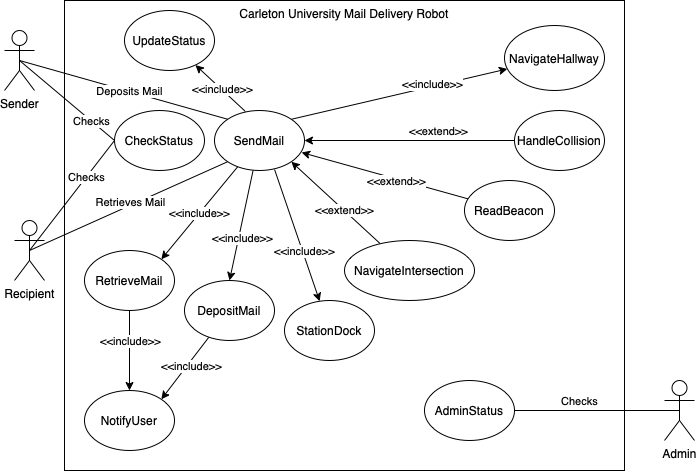
\includegraphics[scale=0.6]{images/UseCaseDiagram.png}
\centering
\end{figure}
\subsubsection{Mail Delivery}
A robot will take mail from Station A in the tunnels to Station B based on user specification.
\subsubsection{Navigation}
A robot can route a path between two locations and then follow walls and navigate intersections until the destination is reached.
\subsubsection{Delivery Status}
Users, both senders and recipients, can check delivery status via a web interface. Delivery status includes whether mail is delivered and last known location of robot.
\subsubsection{Admin Status}
Admins can view full system status via a web interface. Full system status includes last known locations of all robots, reported errors from all robots, and battery levels of beacons. Robots should determine and flag low battery or dysfunctional beacons.
\subsection{Non-Functional Requirements}
\subsubsection{Autonomy}
Autonomy is a fundamental requirement of the mail delivery system. The system should be able to service a users mail delivery request without any additional user or operator involvement.

\begin{description}
    \item[Power Requirements] The robot should operate off batteries which will be able to be recharged autonomously when a robot returns to a station. All onboard device should be powered by these batteries.
    \item[Course Navigation] A robot should be able to determine a general location based on the signals from nearby active beacons. The robot does not need to be able to determine a specific geographic location, but should be able to make correct navigation decisions based on this information.
    \item[Tunnel Navigation] The robot will be able to successfully navigate from point A in the tunnels to point B. The robot should always plot the most direct route from point A to point B. Maximum trip time for the test route should be no longer than one hour. Stretch goals will be defined after further testing. 
    \item[Beacon Maintenance] The amount of beacons used will be kept to a minimum to reduce the initial cost of installation and upkeep. Initially, four beacons per intersection will be used with the goal of reducing it to two and possibly even one.
\end{description}

\subsubsection{Safety}
The robot should not be a public safety risk. The robot should not be capable of knocking over objects in the event of a collision. 

\subsubsection{Robustness}
In the event of a collision, inactive beacons or other obstacles, the robot should still make the best possible attempt at delivering the mail. The robot should be able to be pushed to any location in the tunnels and be able to regain course and continue delivery.

\subsubsection{Affordability}
Each robot should be reproducible within a budget of \$500. A minimal amount of beacons should be used to reduce set-up and operational cost.

\subsubsection{Ease of Use}
A first-time user should be able to quickly navigate the web interface and submit a request or monitor a request. The system should not require any training to use.

\subsubsection{Ease of Setup and Maintenance}
An administrative user will be able to construct and deploy a new robot quickly and without frustration. The target for assembly time is one hour with a stretch goal of forty-five minutes. Replacing parts will require minimal time and effort. Repairing any robot should take no longer than thirty minutes for anticipated failures with a stretch goal of fifteen minutes.

\section{Relationship to Degree Program}
Computer Systems Engineering is a degree program which focuses on "combining hardware and software to design and implement integrated computer systems for applications in such areas as robotics, artificial intelligence, aerospace and avionic systems, multimedia applications and cloud computing". Computer Systems Engineering develops skills in software engineering, analog and digital electronics, computer systems and engineering principles.

This project will involve thoroughly designing and building a system with hardware and software components, following proper engineering principle, and documenting and discussing the process.

A key aspect of the project is proper requirements elicitation and specification, software design and validation and verification. To accomplish this tools such as UML and other system modelling methods will be used. These skills are a focus of \textit{SYSC 3020: Introduction to Software Engineering}.

Furthermore, the robot system will be a distributed concurrent system. The software design will require a communication protocol, multiple threads and a scheduling system. These skills are a focus of \textit{SYSC 3303: Real-Time Concurrent Systems}.

Another aspect of the project is sensors, beacons and other I/O devices. The robot will need to interface with these peripherals and utilize interrupts and other I/O implementation strategies. The entire system is wireless and therefore must operate within power, processing and other constraints. These skills are a focus of \textit{SYSC 3310: Introduction to Real Time Systems}.

The Computer Systems Engineering degree program focuses on developing these skills through designing and implementing systems, such as the one in this project. Over the course of this project, the students will be able to apply these skills and integrate different aspect of the degree program into a single project.


\section{Required Skills}
This project requires a range of skills across subjects. This section will discuss what is required and how the group has the capability to undergo the project.

\subsection{Software Engineering}
The project requires the ability to design, build and thoroughly test software systems. The students in the group have developed the skills required through their degree program, Computer Systems Engineering. The following courses: \textit{SYSC1005: Introduction to Software Development}, \textit{SYSC2004: Object-Oriented Software Development}, and \textit{SYSC2006: Foundations of Imperative Programming} allowed the students to develop a range of knowledge of different programming principles. Furthermore, the students completed a medium-sized software and hardware project in \textit{SYSC3010: Computer Systems Development Project}. This project gave the students experience in developing, testing, and documenting a software project.

\subsection{Distributed Systems}
The project requires designing a system which has distributed components that must communicate between each other. This requires expertise in systems design and communication. The students have experience in working with distributed systems when they developed an elevator system in \textit{SYSC 3303: Real-Time Concurrent Systems}. This previous project involved designing a communication model, scheduling and ensuring that all aspects of the system were robust.

\subsection{Embedded Systems}
The robot is an embedded system with power, processing and other constraints which interfaces with a multitude of peripheral devices, this requires a unique set of programming and engineering skills. The students have experience with these types of systems in \textit{SYSC3310: Intro to Real-Time Systems} where they developed knowledge of embedded systems and different I/O implementations.
%%%%%%%%%%%%%%%%%%%%%%%%%%%%%%%%%%%%%%%%%%%%%%%%%%%%%%%%%%%%%%%%%%%%%%%%%%%%%%%%%%
\chapter{Background}
\section{Project History}
This project was first outlined in 2019 in the paper \textit{Toward Campus Mail Delivery Using BDI}\cite{PatrickPaper} by Chidiebere Onyedinma, Patrick Gavigan and  Babak Esfandiari. The paper explore automated systems utilizing Belief-Intention-Desire system and realized in a real-world environment using iCreate Roombas and ROS. The autonomous mail delivery system was continued in  2020 by another group of students at Carleton University in their project, \textit{Autonomous Mail Delivery Robot in University Tunnels}. This project will be a further continuation towards the goal of a fully autonomous mail delivery system in the Carleton University tunnels.
\section{Robot Operating System}
ROS is a set of libraries and tools for developing robotic applications. ROS is a distributed and modular framework made up of many high quality user contributed ``ROS Packages". ROS uses software nodes and publisher-subscriber model and socket-based communications. The publish-subscribe pattern allows senders, called publishers to categorize messages into classes without knowledge of the receivers, called subscribers. Subscribers subscribe to classes they have interest in and receive only messages of that class. Therefore, developers only need to consider the classes they are subscribing or publishing to, and not all the interactions.
\section{iRobot Create 2}
The iRobot Create 2 is an educational robotic platform designed to be affordable and extensible. It provides a serial interface to allow for specific control of the robots motors and sensors or alternatively the ability to trigger a variety of existing behaviours. 

One such behaviour is the ability to automatically dock with the included charging station. This allows developers to focus on  their specific application and to not need to consider how to implement common behaviours such as charging.

The iRobot Create 2 has built in sensors that are useful for object avoidance and tamper indication. Bumper sensors indicate when there is an obstacle and wheel drop sensors can indicate a ledge has been reached or the robot has been picked up. These built in sensors greatly reduce the assembly complexity of a project using this platform.
 %=================================================================================
\chapter{Methods}
 Other implementations of automated mail delivery use vacuum tubes or conveyor belts. Unfortunately, both of these solutions are infeasible when retrofitting to existing infrastructure. This is where the Carleton University Mail Delivery Robot aims to improve on the existing system of human delivery without any major changes to the existing infrastructure.
\section{Project Management}
\subsection{Timeline}
\begin{table}[H]
\centering
\caption{Proposed Timetable for Completion of the Project Milestones}
\centering
\begin{tabular}[t]{lcc}
\toprule
Milestone&Date\\
\midrule
\textbf{Project Proposal}&\textbf{October 22nd}\\
Basic Robot Functionality&November 18th\\
Basic Robot Autonomy&December 10th\\ 
\textbf{Progress Report}&\textbf{December 10th}\\
Intermediate Robot Autonomy&January 24th\\
\textbf{Final Oral Presentation}&\textbf{January 24th}\\
Full System Demonstration&February 17th\\
\textbf{Final Report Draft}&\textbf{February 28th}\\
\textbf{Poster Fair}&\textbf{March 18th}\\
\textbf{Final Report}&\textbf{April 12th}\\
\bottomrule
\end{tabular}
\begin{tablenotes}
      \small
      \centering
      \item Note: Milestones in bold are hard due dates.
\end{tablenotes}
\end{table}%

\begin{description}
   \item[Basic Robot Functionality] The robot can be controlled by the micro-controller. Wall-following and other scripts can be tested. The robot can read information from the beacons. The web application can be used to send requests.
   
  \item[Basic Robot Autonomy] The robot responds to requests submitted from the web application autonomously. The robot can follow a wall. The robot can determine which beacons are nearby.
  
  \item[Intermediate Robot Autonomy] The robot can receive requests and attempt to navigate to them without assistance, including through intersections. The web application looks functional and is intuitive.
   
   \item[Full System Demonstration] All functional requirements of the system are met.
   
\end{description}
\subsection{Required Components}
\subsubsection{Tunnel Access}
Access to the tunnels at Carleton is ideal for deploying and proper testing of the system. If this proves to be impossible, hallways of a campus building may be used instead.
\subsubsection{Hardware}
\begin{table}[H]
\centering
    \caption{Required Hardware}
    \begin{tabular}{  l  p{8.5cm} r}
        \toprule
\textbf{Item}      
& \textbf{Description} 
& \textbf{Cost} 
\\\hline
iRobot Create 2
& Robot platform
& \$250
\\\hline
Raspberry Pi 4
& Main controller. 4GB model.
& \$68.75
\\\hline
Raspberry Pi Zero W
& Boot controller
& \$20.94
\\\hline
Buck converter
& Regulate Create 2 robot output voltages to Pi input voltage. Max input of up to 20.5V. Output 5V and at least 3A.
& ~\$5 x2
\\\hline
Inductor
& 2.2mH 1.5A inductor (Ex. Murata 1422514C). Required to use main motor driver on Create 2 robot.
& ~\$6
\\\hline
Wall sensor
& Currently Sharp IR sensors.
& \$15 x2
\\\hline
Bluetooth beacon
& To allow robot to locate intersections. Currently AprilBeacon N04.
& \$10 per
\\\hline
iRobot base station
& To allow robot to charge. One base station is included with each Create 2 robot.
& \$80 per
\\
        \bottomrule
    \end{tabular}
    \begin{tablenotes}
      \small
      \centering
      \item Note: Some cost values are estimates. Tax and shipping is not included.
      \item Note 2: All items are cost per robot except beacons and stations.
\end{tablenotes}
\end{table}

\subsection{Project Risks}
The table below outlines the project risks and mitigation strategies.

\begin{table}[H]
\centering
    \caption{Project Risks and Mitigation Strategies}

    \begin{tabular}{  l  p{8cm}}
        \toprule
\textbf{Project Risk}      
& \textbf{Mitigation strategy} 
\\\hline
Hardware Failure 
& All critical hardware will be replaceable within a reasonable window of time. For items such as beacons or other low cost components, multiple components can be purchased for redundancy. For other components, availability and cost will be considered so that they may be replaced within budget. 
\\\hline
Unable to Access Testing Sites 
& Each group member has access to their own testing equipment. In the event that a testing site cannot be accessed, each member will be able to test the system independently in their own testing area.
\\\hline
The ``Bus Factor"   
& In the event that one group member is unable to continue the project, this should not cause any of their work to be lost. To prevent this all team members will document their work thoroughly and continuously. All work will be stored on the GitHub repository or other cloud-based version controlled solutions. Furthermore, both students will always be participating in all aspects of the project. To facilitate this, pull requests will be made for new additions and code reviews will be conducted before they are merged.
\\\hline
Over-budget/Inflating Project Costs
& Hardware solutions to problems should be simple, easily reproduce-able and cheap. This should allow any needed hardware additions to be reproduced on both robots and any hardware failures to be replaced without going over budget.
\\
        \bottomrule
    \end{tabular}
\end{table}


%=================================================================================

\section{Project Planning and Organization}
The previous team struggled with closely collaborating on all aspects of the project and integrating individual work together. The result of this is that their completed project is disjointed and it is unclear how to run it all at once. In order to avoid these issues, the following project management specific principles should be met:
\begin{itemize}
\itemsep0em 
    \item Every team member generally understands all aspects of the project
    \item To-do tasks are clearly laid out and who is currently working on what is visible
    \item A historical view of progress is available for review
    \item A strong emphasis on agile development principles
    \item No completely independent changes
\end{itemize}
\subsection{Issue Tracking}
To ensure all necessary tasks are tracked, every todo item will be created as a GitHub issue. Issues will be assigned to project member(s) so that it is clear who is working on what at which time. In addition, an individual member can quickly filter only their issues. As well, only issues without an assignee can be filtered in order to see if there are any issues that are being ignored or forgotten about. This should decrease the likelihood that important issues are missed and make it much easier to view who is working on what.
\subsection{Issue Filtering}
Issues also have the ability to be labelled for quick filtering. One custom label that will be implemented is a “have discussion” label. This will be used during team meetings to quickly pull up a list of what team members want to discuss. This will ensure that issues that need a team discussion won’t be forgotten about and potentially pushed into the future.
\subsection{Weekly Project Board}
GitHub issue tracking will be integrated with a weekly GitHub project board. This will show which issues are being worked on for the week in an agile development Kanban view. This is an ideal view for quickly getting an idea of project progress, making it easier and faster to make decisions for what to work on or while reviewing the past week's progress. In addition, we will automate the GitHub project board to match actions in the repository. For example, automatically moving an issue to the “done” column and closing it when the linked pull request is approved and merged. This will reduce project management overhead and free up time to focus on coding. Past boards will remain view-able so project management issues can be identified and solutions implemented on a recurring, agile basis.
\subsection{Code Review and Collaboration}
The GitHub repo will be set up to prevent a merge to main without approval from a different team member. This will force code review and increase general understanding of the project for all team members. Importantly, this will prevent only a single team member from having knowledge of a piece of code.
\subsection{Miscellaneous}
The project management goal will be for any issue to be worked on by any member interchangeability. It is also vital that our project management strategy is reviewed on a recurring basis to ensure that it is working. As a result, the above guidelines are a starting implementation and will likely change in an agile manner as improvements are discovered.

%=================================================================================

\section{Build Automation System}

Currently, there are five repositories with code for the project.
\begin{enumerate}
\itemsep0em 
\item WebServices-Client
\item WebServices-Server
\item Roomba
\item Distance-from-rssi
\item Web-App
\end{enumerate}
Each requires different dependencies and methods for building. This makes it difficult to develop
and build the software for all components.


\subsection{Repository Structure}
There is not a need to create multiple repositories for different components of the project since no
component is completely independent of one another. Furthermore, by organizing all
components into a single repository, we have a “single source of truth”. This will make it easier
to more closely collaborate, share and verify code, and refactor when needed.
The organization of the project will be a single mono-repo with each component being a
top-level directory.

\subsection{Github Actions (Continuous Integration Pipeline)}
In order to simplify the building process for all software components of the system a GitHub
actions scheme will be set-up to automate the build process. On a push the GitHub action will
automatically build all the components using docker. Furthermore, this system can run unit tests
and integration tests, verifying the code on every push. With this in place, all the components of
the system can be kept up-to-date and tested continuously.
\subsection{Docker}
Docker will be used to package the software components with the libraries and dependencies
required to run them in any environment. It will allow easy sharing of source code without having
to set-up or change our development environments. With a DockerFile setup the code of any
component can be built through the GitHub action scheme or locally

%=================================================================================

\section{Web Application}
The web application is the user interface for the entire mail delivery system. It should primarily allow users to:
\begin{itemize}
\itemsep0em 
\item Request a delivery robot
\item Make delivery requests
\item Monitor delivery requests
\end{itemize}

The web application should:
\begin{itemize}
\itemsep0em 
\item Look polished
\item Be intuitive to users
\item Be secure from malicious activity
\item Be available to users through any web browser
\item Function properly on a mobile device
\end{itemize}
\subsection{Angular}
The web application will be built using Angular, a typescript-based web application framework. 
\begin{description}
   \item[PWA] Angular allows for the creation of progressive web apps (PWA) which are applications delivered through the web but intended to deliver app-like experiences across any platform.
   \item[Code Generation] Angular has many tools for code generation, allowing for rapid creation of polished looking interfaces.
   \item[Templates] Angular has a powerful template syntax which allows for creation of complex UIs without having to reinvent the wheel at every step.
\end{description}
\subsection{Web Server}
The web application will run in conjunction with a web server that will relay requests to an appropriate robot. Constant communication with the robots in the tunnels is impossible due to the lack of internet access, therefore, communication is kept very simple.

The web server will send http requests with Deliver, Recall and Check commands. These encompass all possible commands that the web server would give to the robot. A `Deliver' requires two locations and a userID, which commands the robot to navigate to location A, then location B. A `Recall' requires a location and a userID, it requests the robot to navigate to a single location. A `Check' requires a userID, it requests the status of the robot. All above commands require a userID as the user who requests the action is recorded. This can later be extended to provide user authentication.

The robot has a single http message format, Status. This includes a location, a robotID and a Status. Every time the robot receives a command, it will respond with a Status, the status will determine if the robot can complete the command, along with its location and id for tracking. The robot will send a status update when it arrives at a location or when it experiences an error. The different status messages the robot can send are included in the table below.

\begin{table}[H]
\centering
\caption{Communication Protocol Table}
\centering
\begin{tabular} { | p{2cm} | p{2cm} | p{2cm} | p{8cm} | }
\hline
Sender & Receiver & Message & Parameters \\
\hline
Server & Robot & Deliver & \{``sourceLocation": int, ``destLocation": int, ``userId": int\} \\
\hline
Server & Robot & Recall & \{``Location": int, ``userId": int\} \\
\hline
Server & Robot & Check & \{``userId": int\} \\
\hline
Robot & Server & Status & \{``Location": int, ``robotId": int, ``Status":int\} \\
\hline
\end{tabular}
\end{table}%

\begin{table}[H]
\centering
\caption{Robot Status}
\centering
\begin{tabular} { | p{2.5cm} | p{12cm} | }
\hline
Status& Description \\
\hline
Available & The robot is charged and available to complete a delivery. \\
\hline
InProgress & The robot is currently completing a delivery or recall request. \\
\hline
Complete & The robot has completed a delivery or recall request. \\
\hline
Charging & The robot is charging and is unable to complete a delivery request. \\
\hline
BeaconFault & The robot has encountered a beacon it cannot communicate with or is low battery. The location will be the beaconID. \\
\hline
Stuck & The robot cannot continue normal operation. \\
\hline
\end{tabular}
\begin{tablenotes}
      \small
      \centering
      \item Note: Every robot status message has a location attached. By default it is the robot's location.
\end{tablenotes}
\end{table}%

\begin{figure}[H]
\caption{Web Server Communication Sequence Diagram}
\centering
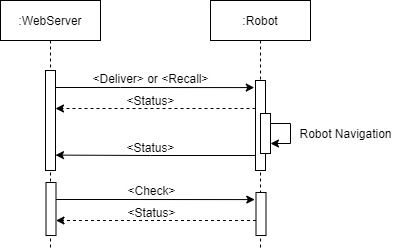
\includegraphics[scale=0.8]{images/CommunicationSequenceDiagram.jpg}
\centering
\end{figure}

%=================================================================================

\section{Navigation}
An apparent success of the previous mail delivery robot project, \textit{Autonomous Mail Delivery Robot in University Tunnels}, was their wall following algorithm and hardware. This will be replicated and implemented again as the primary navigation method for the robot. In the event the IR sensors prove to be inconsistent, they will be replaced with ultrasonic sensors but will still be implemented with the same algorithm. When it comes to intersections, wall fallowing can no longer be used. For more information on how intersection navigation will work, see the section on Bluetooth beacons.

The second half of navigation, routing, will be implemented with a simple dictionary. There are a relatively small number of start and end points on campus, so the ideal route between every point can simply be loaded into a dictionary. This is not ideal for scaling up to a larger project; however, a more complicated routing algorithm is out of scope. The dictionary method is more than sufficient for this project.

%=================================================================================

\section{Robot Operating System}
ROS will function as the software platform that will be the brains of our robot. Through the ROS subscriber-publisher model, the gathering of information and the use of this information can be decoupled. In our project for example, scripts which read sensor information and the scripts which control navigation of the robot can then also be decoupled. This will allow us to easily re-use scripts from the previous work done on the project and integrate seamlessly.

The following information needs to be gathered by the robot:
\begin{itemize}
\itemsep0em 
\item Requests from the server
\item IR sensor data for wall following
\item Beacon data for determining course
\item Bumper Data for determining collision
\end{itemize}

Using the information gathered, the robot then needs to make navigational decisions. The following navigational decisions need to be made by the robot:
\begin{itemize}
\itemsep0em 
\item Plotting a route from Point A to Point B
\item Following a wall to maintain course
\item Making turns at intersections
\item Navigating around obstacles after collisions
\item Docking for charging
\end{itemize}

Each of the items above can be broken into separate ROS scripts, some of which we can reuse from previous work done on this project.
\subsection{Reuse of ROS Scripts}
The following ROS scripts have been used in the previous project and will be reused.
\begin{table}[H]
\centering
\caption{Reusable ROS Scripts}
\centering
\begin{tabular} { | p{4cm} | p{8cm} | }
\hline
Script Name & Description \\
\hline
IRDistanceCalc.py & Reads the IR Sensors and determines a distance from the wall. This will be used to enable the robot to follow a wall. \\
\hline
BumperSensor.py & Reads the status of the robot's bumper. This will be used to determine when the robot has collided with an object. \\
\hline
driverBluetooth.py & Reads bluetooth information from the environment. This will be used to read data from the beacons and allow the robot to determine a course. \\
\hline
actionTranslator.py & Converts roomba movement messages into iRobot compatible messages. \\
\hline
\end{tabular}
\end{table}%

\subsection{Additional ROS Scripts}
The following ROS scripts will be created for this project.
\begin{table}[H]
\centering
\caption{ROS Scripts}
\centering
\begin{tabular} { | p{4cm} | p{8cm} | }
\hline
Script Name & Description \\
\hline
ReceiveRequest.py & Receives and stores requests received from the web server.\\
\hline
PlotNavigation.py & Determines a route from point A to point B of the current request. This involves determining all the intersections to turn at. This can be recalculated if the robot gets lost.\\
\hline
RobotDriver.py & Uses the plotted navigation map, beacon information and IR sensors to follow a wall until the desired intersection and then makes a turn. \\
\hline
HandleCollision.py & Uses the bumper sensor to navigate around an obstacle after a collision.\\
\hline
Captain.py & Uses the navigation data and the navigation map to keep track of the robot with relation to the map. Determines if the robot is off course and the map needs to be recalculated or if beacons are missing or non-functional. \\
\hline
UpdateStatus.py & Sends an update to the web server with the current location of the robot.\\
\hline
DockRobot.py & Navigates to a docking station and charges the robot.\\
\hline
\end{tabular}
\end{table}%

\subsection{ROS System Overview}
The ROS scripts are each independent nodes which publish and subscribe to different topics. Should a single node be non-functional, crash or its related sensor be offline, the rest of the nodes can keep operating. Each node subscribes to the topic it requires to function and publishes its output to the topic for other nodes to use.

The ROS Node Map below outlines how the nodes are related in the system. The Requests topic is used to store the requests which the robot receives from the web server, these requests are used by the PlotNavigation node to update the NavigationMap topic. The Navigation topic is used to store the navigational data from all the robots sensors. The robot driver reads Navigation topic and the NavigationMap to determine how the robot should move. The Captain node reads the Navigation and NavigationMap and updates the map to adjust course, detect errors and keep track of where the robot is. The UpdateStatus node uses the NavigationMap data to update the web server of the robots status when possible or requested. The HandleCollision node goes around the RobotDriver in the event of a collision and it determines the course until the collision is avoided.

\begin{figure}[H]
\caption{ROS Node Map}
\centering
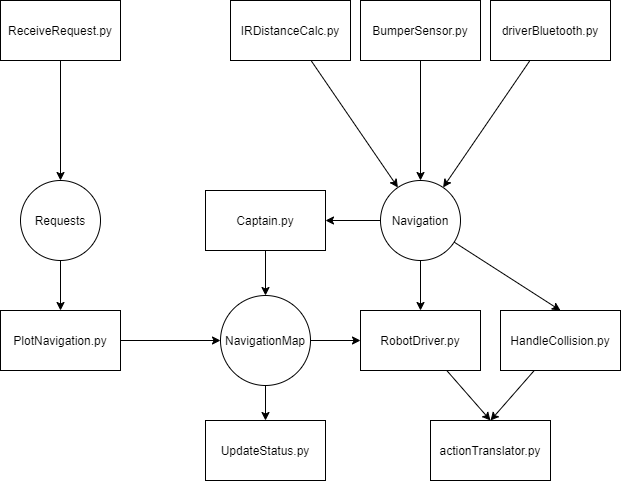
\includegraphics[scale=0.6]{images/ROSNodeMap.png}
\centering
\end{figure}

%=================================================================================

\section{Power Subsystem}
A vital nonfunctional requirement to ensure project longevity is easy of setup and maintenance. In pursuit of this goal, electronics on top of the iRobot Create 2 should be powered solely by the iRobot's battery. This will greatly simplify power delivery and charging compared to alternatives such as a secondary battery pack.

\subsection{Power Requirements}
The power requirements for the two possible significant power draws are as follows:
\begin{description}
    \item[Raspberry Pi 4] The recommended power supply for a Raspberry Pi 4 is 5V at 3A\cite{Pi4Specs} for a total of 15W. This allows for at least 1A to go to attached sensors and accessories which is far more than any potential sensors this project will use.
    \item[Raspberry Pi Zero W] The Raspberry Pi Zero W uses a maximum of around 230mA at 5V (1.15W) during heavy loads and near half that for more typical loads \cite{PiZeroPower}.
\end{description}

\subsection{Power Sources}
The iRobot Create 2 can supply power in the following two ways. Note: this does not apply to the iRobot Create 1, our system design will assume an iRobot Create 2 but a non standard testing setup will be implemented on the iRobot Create 1. 
\begin{description}
    \item[Serial Port] The iRobot Create 2 has a serial port capable of providing 0.2A at 10V-20.5V for a maximum rated capacity of 2W \cite{BatterySpecs}. This serial port is constantly powered when the iRobot Create 2 is powered. 
    \item[Motor Driver] The iRobot Create 2 has several motor drivers, the main one capable of providing 1.45A at 12V for a maximum rated capacity of 17W \cite{BatterySpecs}. A 2.2mH 1.5A inductor is required to use the main motor driver.
\end{description}

\subsection{Power Plan}
The main motor driver with a rated capacity of 17W is more than capable of powering any electronics that could be implemented for this project. A simple buck converter circuit to bring the voltage down to 5v for the Raspberry Pi 4 can provide more amperage (3.4A) than the standard Pi 4 power supply (3A). This means that a Pi 4 powered via the motor driver can function as if plugged into the wall along with any sensors that work with a typical Pi 4 setup. The one drawback is that the main motor driver is not powered on boot until a command is sent over the serial cable. In order to use the motor driver to power the Pi 4, an additional lightweight controller is needed to run off the always powered serial port. This port provides more than enough power for a Raspberry Pi Zero W or similar microcontroller, although it is insufficient for the Pi 4. As with the motor driver, a simple buck converter circuit attached to the serial port provides more power (5V 400mA) than is needed to power the Pi Zero W (5V 230mA). The main purpose of the Pi Zero W is to run a boot sequence to power on the Pi 4 and from that point, the Pi 4 will be the primary controller.

%=================================================================================

\section{Bluetooth Beacons}
The Bluetooth beacons are part of the positioning system for the mail delivery robot. They may not be the sole positioning method. The Bluetooth beacons should allow the robot to:
\begin{itemize}
\itemsep0em 
\item Determine a rough location along a path
\item Connect to the beacon from a reasonable distance
\item Check the battery level of the beacon
\end{itemize}
\subsection{Experimentation}
Three April N04 beacons were placed in a straight line, approximately five meters apart in separate rooms. Proximity and signal noise (rssi) were measured using the manufacturers app on an iPhone 13 Pro. The beacons tx power was set to the maximum (4dB).
\begin{description}
    \item[Location Accuracy] The proximity values for the three beacons consistently were in the correct order based on phone distance to each beacon. When considering an individual beacon, the proximity values frequently changed with up to a 50\% margin of error. This suggests the relative values from multiple beacons are reliable; however, the individual proximity values are not. That being said, an individual value can be used to determine if approaching or departing from a beacon. To get the most accurate proximity value, several samples, for example five, will be taken and then averaged with the outliers discarded. The exact number of samples will be decided on based on testing during implementation. In addition, there was an observed issue where the value will rapidly ramp up or down without any phone movement. To combat this, a maximum standard deviation will be used to discard this behaviour. 
    \item[Connection Distance] Proximity values were received from the highest distance tested, approximately fifteen meters without line of sight. In the tunnels with less obstruction, the actual distance is likely to be much higher; theoretically up to 30 meters according to the manufacturers documentation.
    \item[Beacon Battery] Battery values for the beacons are readable through the app. These values are also readable using the SDK. One limitation is the app cannot reliably get additional information, such as battery, when the beacon is further than approximately five meters away. It is unclear if the SDK has this same limitation although five meters should be sufficient regardless. 
\end{description}
\subsection{Beacon Placement}
In order to minimize the number of beacons, it is ideal for the robots navigation system to not require connection to a beacon at all times. Since the tunnels have few intersections, the main purpose of the beacons should be to help the robot navigate down the correct hallway at an intersection. Based on the experimental results, relative proximity values for two beacons are reliable. In addition, the robot should be able to determine if it is approaching or departing from a beacon. One possible setup for beacon placement is putting a beacon slightly down each tunnel at an intersection. The robot can then know it is approaching an intersection when the beacon in its current tunnel comes into range. This will let the robot know what intersection it is approaching and from which tunnel. Based on that information, the robot should be able to determine if it needs to go straight or turn after it stops detecting the wall it is following. The relative proximity values for the beacons should allow the robot to determine if it successfully traversed the intersection or if it needs to turn around and try again. It is possible that only two beacons are needed for a standard 4 direction intersection to determine the same information. In addition, a single beacon with passive RFID tags along the walls right before intersections is likely a lower cost alternative that may also perform more reliably.

%%%%%%%%%%%%%%%%%%%%%%%%%%%%%%%%%%%%%%%%%%%%%%%%%%%%%%%%%%%%%%%%%%%%%%%%%%%%%%%%%%

\renewcommand{\bibname}{References}
\begin{thebibliography}{AAA}
\bibitem{PatrickPaper} C. Onyedinma, P. Gavigan, and B. Esfandiari, “Toward Campus Mail Delivery Using BDI,” Journal of Sensor and Actuator Networks, vol. 9, no. 4, p. 56, Dec. 2020.
\bibitem{Pi4Specs} “Raspberry Pi 4 Model B specifications,” {\em Raspberry Pi}. https://www.raspberrypi.com/products/raspberry-pi-4-model-b/specifications/ (accessed Oct. 13, 2021).
\bibitem{PiZeroPower} Alex, “How much power does Pi Zero W use?,” {\em RasPi.TV}, Mar. 01, 2017. https://raspi.tv/2017/how-much-power-does-pi-zero-w-use (accessed Oct. 14, 2021).
\bibitem{BatterySpecs} “Battery Power from Create 2,” {\em iRobot Education}. https://edu.irobot.com/learning-library/battery-power-from-create-2 (accessed Oct. 14, 2021).
\end{thebibliography}
% If you have your general bibliography in a separate file mybib
% and you wish to use the plain style (see BIBTeX)
%    \bibliographystyle{cacm}
%    \bibliography{mybib}
    \addcontentsline{toc}{chapter}{\bibname}
    
%%%%%%%%%%%%%%%%%%%%%%%%%%%%%%%%%%%%%%%%%%%%%%%%%%%%%%%%%%%%%%%%%%%%%%%%%%%%%%%%%%

% Add appendices now.
\appendix


\end{document}
